In this Section, the results of the application of the mulitclass kernel perceptron algorithm, presented in the theory section above, on the classification of handwritten digits are presented. In the present work, six multiclass predictors with polynomial kernels from degree $p=1$ up to degree $p=6$ are trained on the MNIST training set $S$. For all the six multiclass predictors, $N_{epoch} = 10$ cycles over random permutations of the training set $S$ are performed. As there are three different ways (see theory section) to retrieve binary predictors that underly the multiclass predictors, for each degree $p$ of the polynomial kernel, in effect three multiclass predictors are trained. Subsec.~\ref{subsec:bin_pred} regards the training of binary predictors for the three different approaches. Then, the combination of these binary predictors to obtain multiclass predictors according to the multiclass kernel perceptron algortihm is object of Subsec.~\ref{subsec:multi_pred}. Finally, in Subsec.~\ref{subsec:best_pred}, the obtained multiclass predictors are ranked according to their test error rates on the MNIST test set $D$. 

\subsection{Binary Predictors}\label{subsec:bin_pred}
As explained in Sec.~\ref{sec:theory}, the training of binary predictors is the foundation of the multiclass kernel perceptron. In the present work, the three different binary predictor types $\vec{\alpha}_{fin}$, $\langle \vec{\alpha} \rangle$, and $\vec{\alpha}_{min}$ are retrieved from the binary kernel perceptron alogrithm. For example, in Fig.~\ref{}, the training error rates for the binary prediction of digit $a=5$ using different degrees $p$ of the polynomial kernel are displayed. The corresponding test error rates are reported in Fig.~\ref{}. 

\begin{figure}[h!]
    \begin{subfigure}[t]{0.49\textwidth}
        \centering
        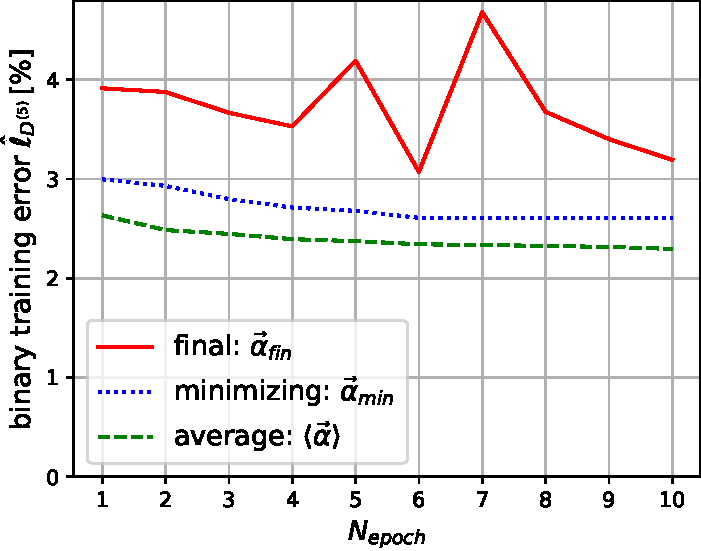
\includegraphics[width=\linewidth]{bin_pred/training_digit=5_deg=1.pdf} 
        \caption{$p = 1$}
    \end{subfigure}
    \hfill
    \begin{subfigure}[t]{0.49\textwidth}
        \centering
        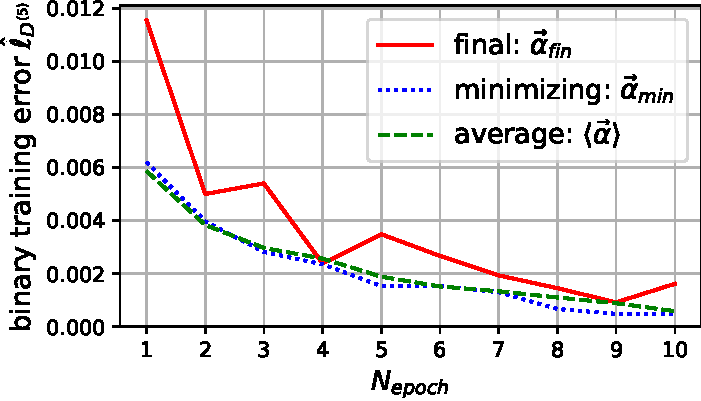
\includegraphics[width=\linewidth]{bin_pred/training_digit=5_deg=2.pdf} 
        \caption{$p = 2$}
    \end{subfigure}
    \par\bigskip
        \begin{subfigure}[t]{0.49\textwidth}
        \centering
        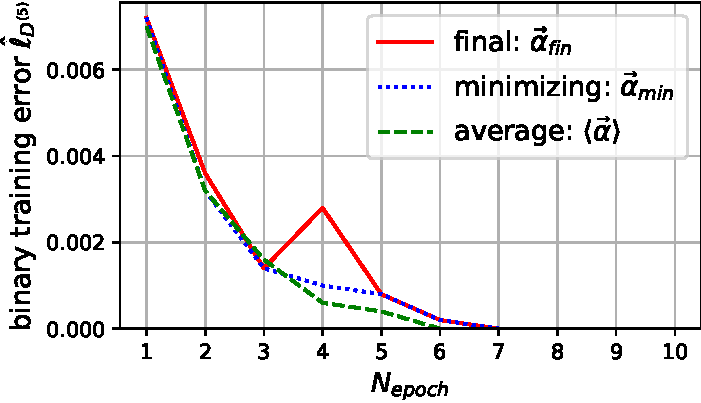
\includegraphics[width=\linewidth]{bin_pred/training_digit=5_deg=3.pdf} 
        \caption{$p = 3$}
    \end{subfigure}
    \hfill
    \begin{subfigure}[t]{0.49\textwidth}
        \centering
        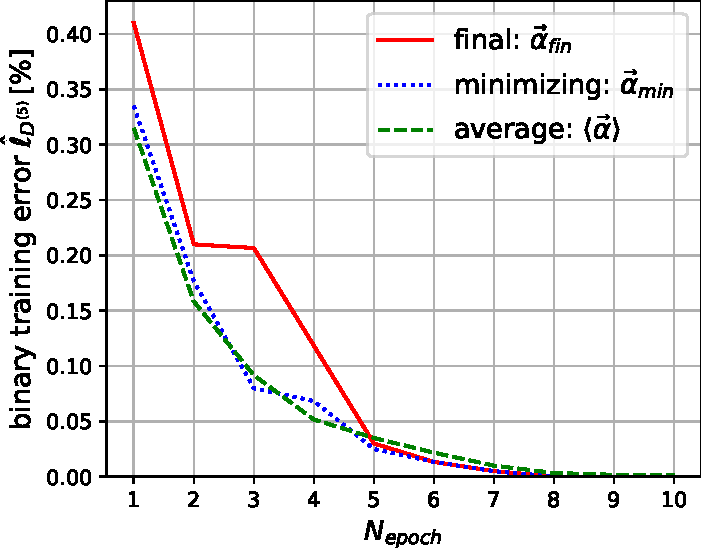
\includegraphics[width=\linewidth]{bin_pred/training_digit=5_deg=4.pdf} 
        \caption{$p = 4$}
    \end{subfigure}
    \par\bigskip
        \begin{subfigure}[t]{0.49\textwidth}
        \centering
        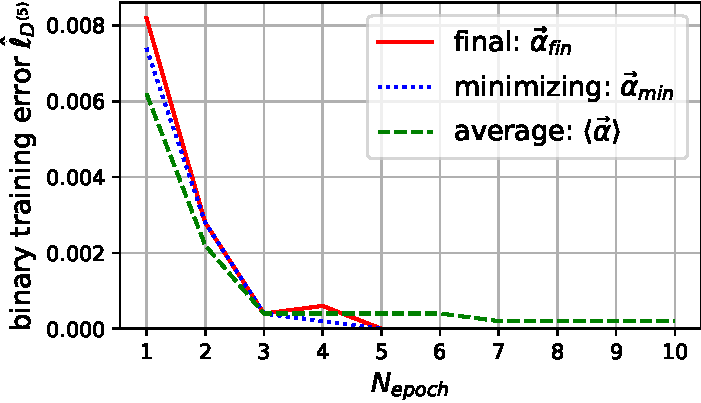
\includegraphics[width=\linewidth]{bin_pred/training_digit=5_deg=5.pdf} 
        \caption{$p = 5$}
    \end{subfigure}
    \hfill
    \begin{subfigure}[t]{0.49\textwidth}
        \centering
        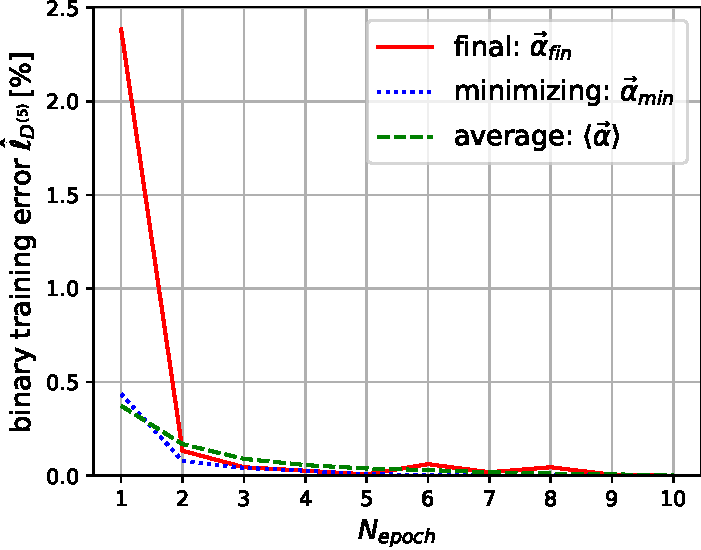
\includegraphics[width=\linewidth]{bin_pred/training_digit=5_deg=6.pdf} 
        \caption{$p = 6$}
    \end{subfigure}
    \caption{training error rates}
\end{figure}

\begin{figure}[h!]
    \begin{subfigure}[t]{0.49\textwidth}
        \centering
        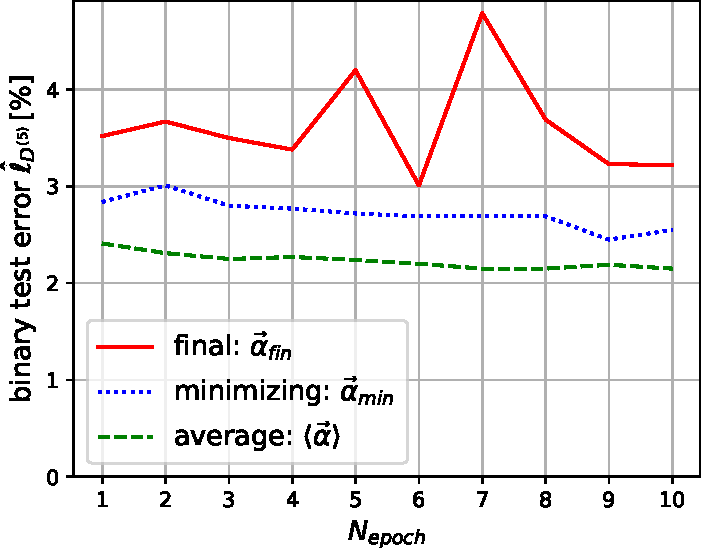
\includegraphics[width=\linewidth]{bin_pred/test_digit=5_deg=1.pdf} 
        \caption{$p = 1$}
    \end{subfigure}
    \hfill
    \begin{subfigure}[t]{0.49\textwidth}
        \centering
        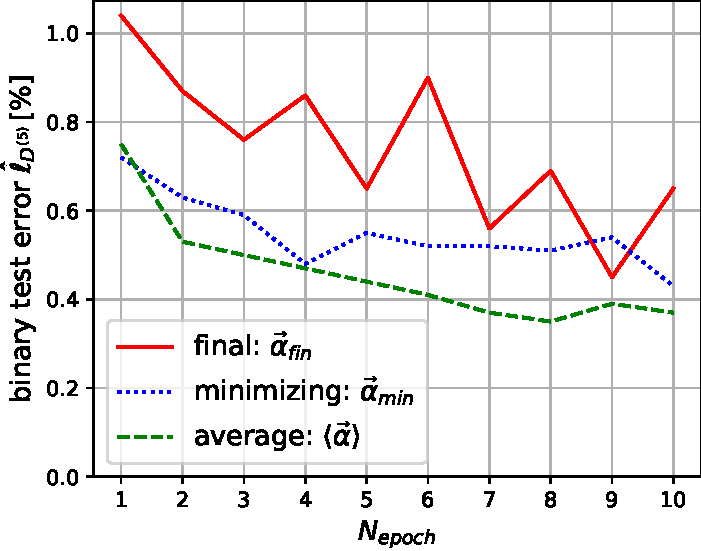
\includegraphics[width=\linewidth]{bin_pred/test_digit=5_deg=2.pdf} 
        \caption{$p = 2$}
    \end{subfigure}
    \par\bigskip
        \begin{subfigure}[t]{0.49\textwidth}
        \centering
        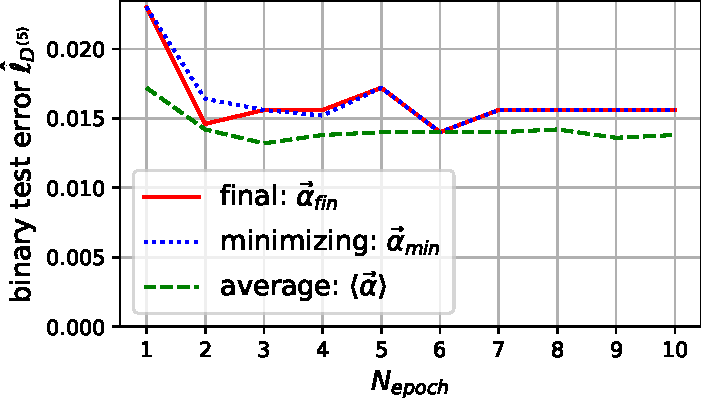
\includegraphics[width=\linewidth]{bin_pred/test_digit=5_deg=3.pdf} 
        \caption{$p = 3$}
    \end{subfigure}
    \hfill
    \begin{subfigure}[t]{0.49\textwidth}
        \centering
        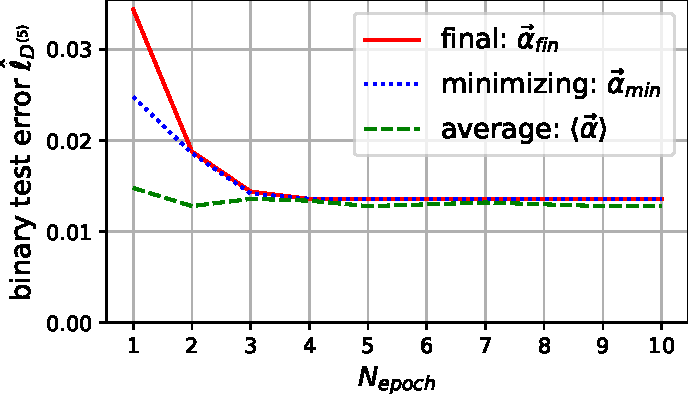
\includegraphics[width=\linewidth]{bin_pred/test_digit=5_deg=4.pdf} 
        \caption{$p = 4$}
    \end{subfigure}
    \par\bigskip
        \begin{subfigure}[t]{0.49\textwidth}
        \centering
        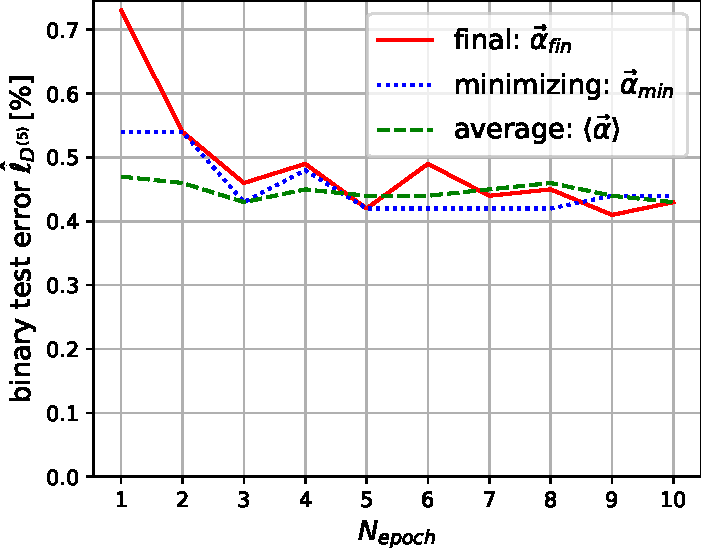
\includegraphics[width=\linewidth]{bin_pred/test_digit=5_deg=5.pdf} 
        \caption{$p = 5$}
    \end{subfigure}
    \hfill
    \begin{subfigure}[t]{0.49\textwidth}
        \centering
        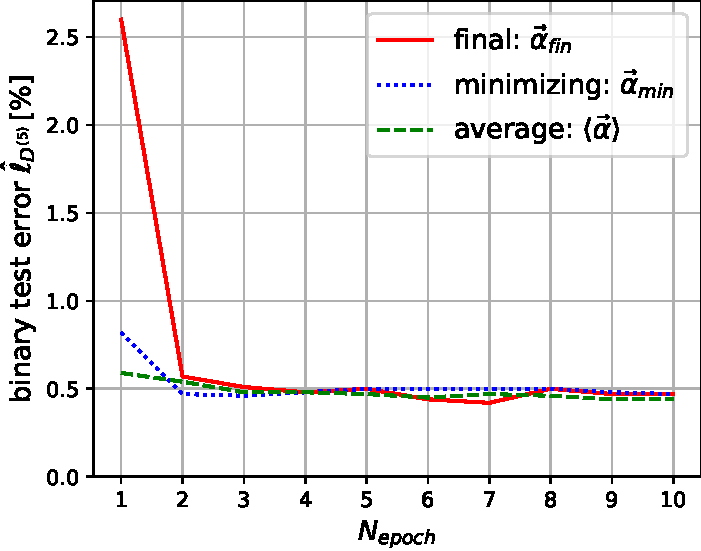
\includegraphics[width=\linewidth]{bin_pred/test_digit=5_deg=6.pdf} 
        \caption{$p = 6$}
    \end{subfigure}
    \caption{test error rates}
\end{figure}

\subsection{Multiclass Predictors}\label{subsec:multi_pred}

\begin{figure}[h!]
    \begin{subfigure}[t]{0.49\textwidth}
        \centering
        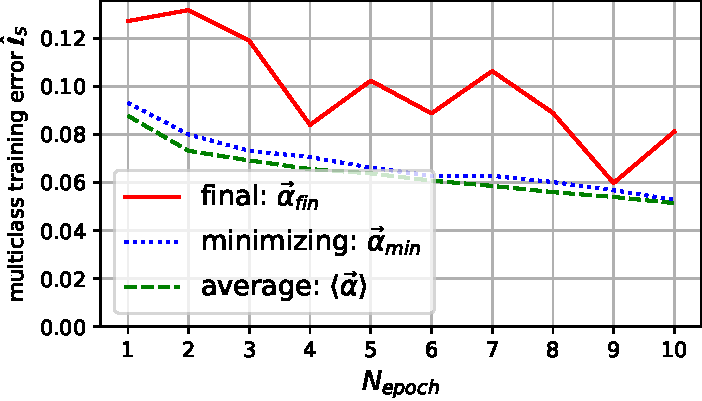
\includegraphics[width=\linewidth]{performance/training_deg=1.pdf} 
        \caption{$p = 1$}
    \end{subfigure}
    \hfill
    \begin{subfigure}[t]{0.49\textwidth}
        \centering
        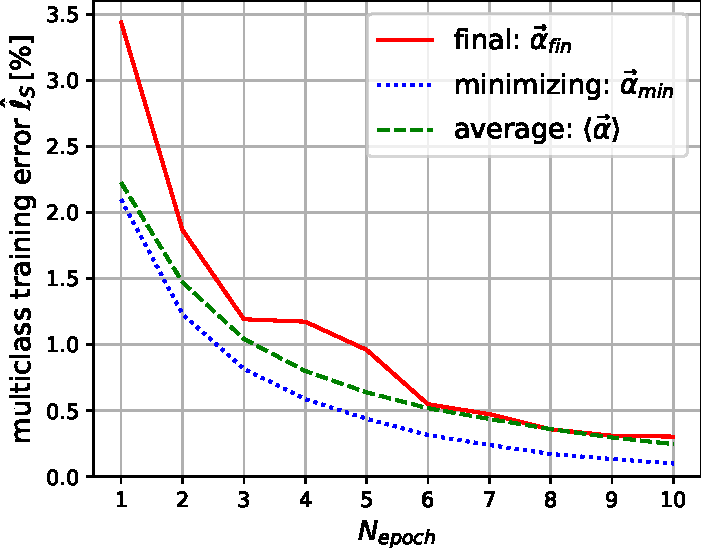
\includegraphics[width=\linewidth]{performance/training_deg=2.pdf} 
        \caption{$p = 2$}
    \end{subfigure}
    \par\bigskip
        \begin{subfigure}[t]{0.49\textwidth}
        \centering
        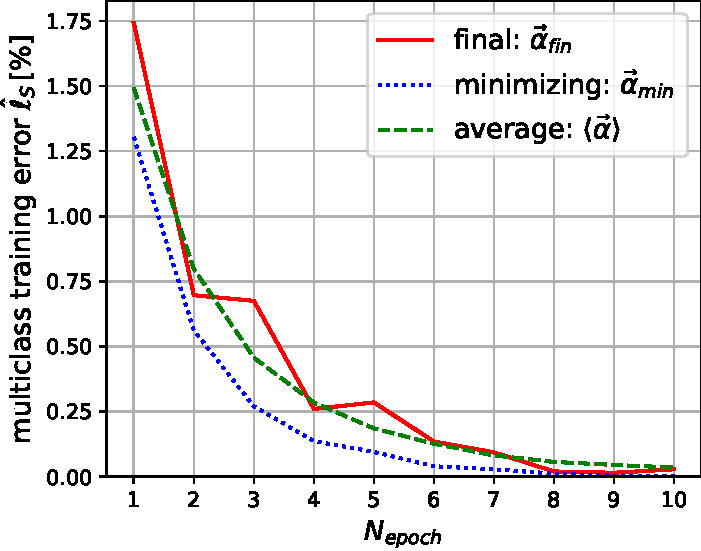
\includegraphics[width=\linewidth]{performance/training_deg=3.pdf} 
        \caption{$p = 3$}
    \end{subfigure}
    \hfill
    \begin{subfigure}[t]{0.49\textwidth}
        \centering
        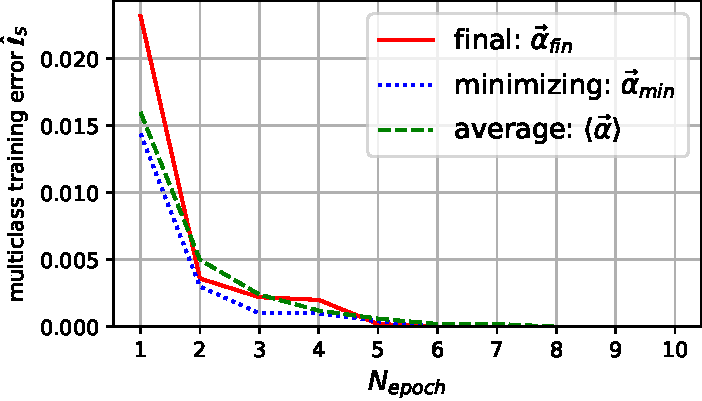
\includegraphics[width=\linewidth]{performance/training_deg=4.pdf} 
        \caption{$p = 4$}
    \end{subfigure}
    \par\bigskip
        \begin{subfigure}[t]{0.49\textwidth}
        \centering
        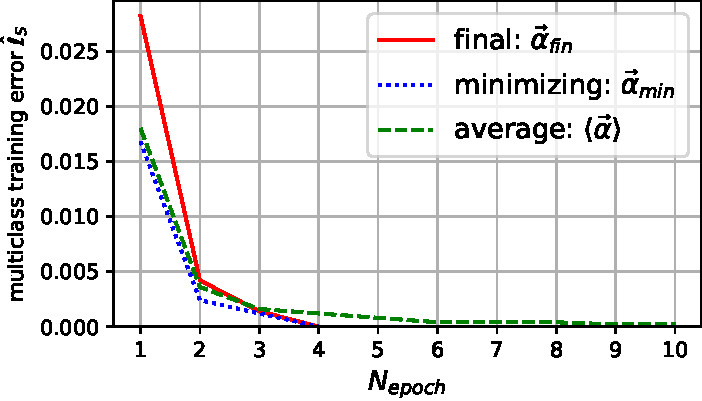
\includegraphics[width=\linewidth]{performance/training_deg=5.pdf} 
        \caption{$p = 5$}
    \end{subfigure}
    \hfill
    \begin{subfigure}[t]{0.49\textwidth}
        \centering
        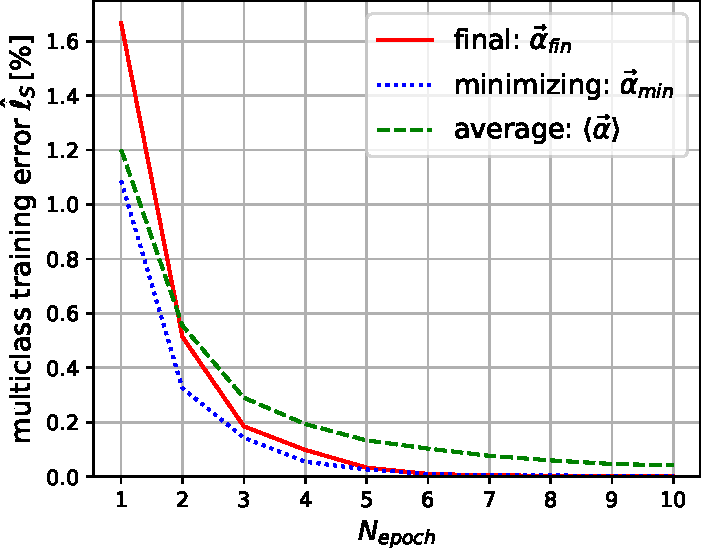
\includegraphics[width=\linewidth]{performance/training_deg=6.pdf} 
        \caption{$p = 6$}
    \end{subfigure}
    \caption{training error rates}
\end{figure}

\begin{figure}[h!]
    \begin{subfigure}[t]{0.49\textwidth}
        \centering
        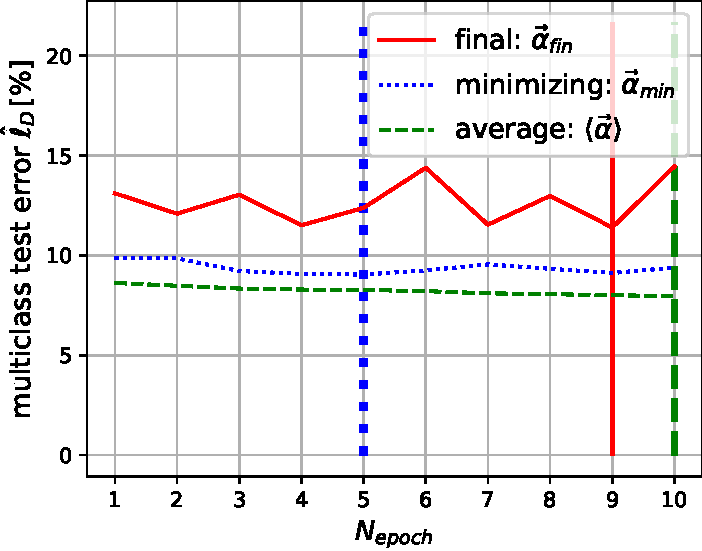
\includegraphics[width=\linewidth]{performance/test_deg=1.pdf} 
        \caption{$p = 1$}
    \end{subfigure}
    \hfill
    \begin{subfigure}[t]{0.49\textwidth}
        \centering
        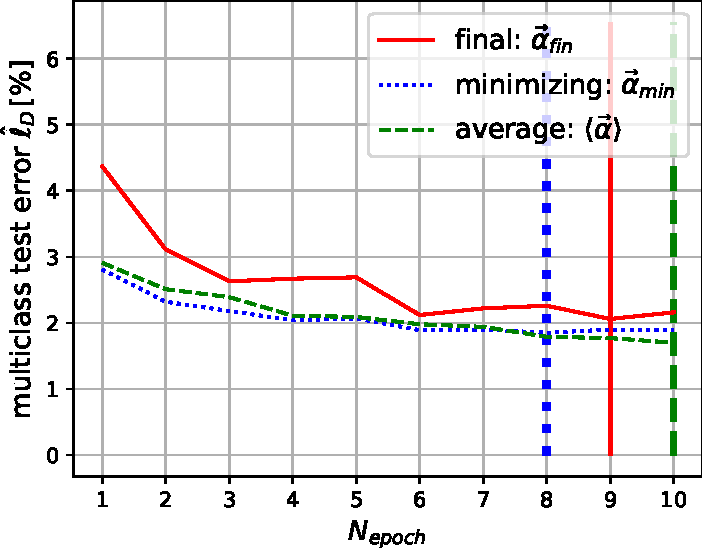
\includegraphics[width=\linewidth]{performance/test_deg=2.pdf} 
        \caption{$p = 2$}
    \end{subfigure}
    \par\bigskip
        \begin{subfigure}[t]{0.49\textwidth}
        \centering
        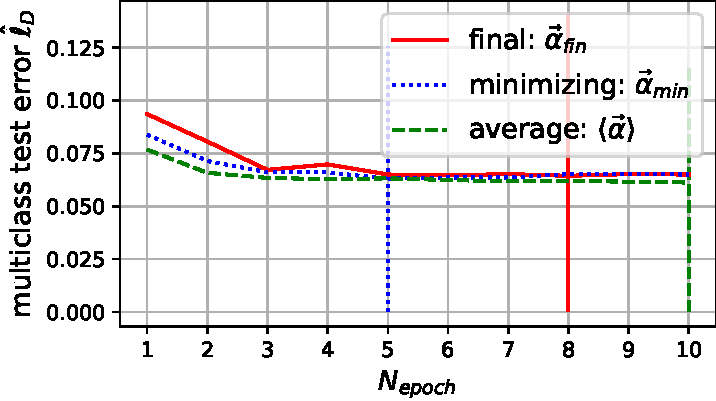
\includegraphics[width=\linewidth]{performance/test_deg=3.pdf} 
        \caption{$p = 3$}
    \end{subfigure}
    \hfill
    \begin{subfigure}[t]{0.49\textwidth}
        \centering
        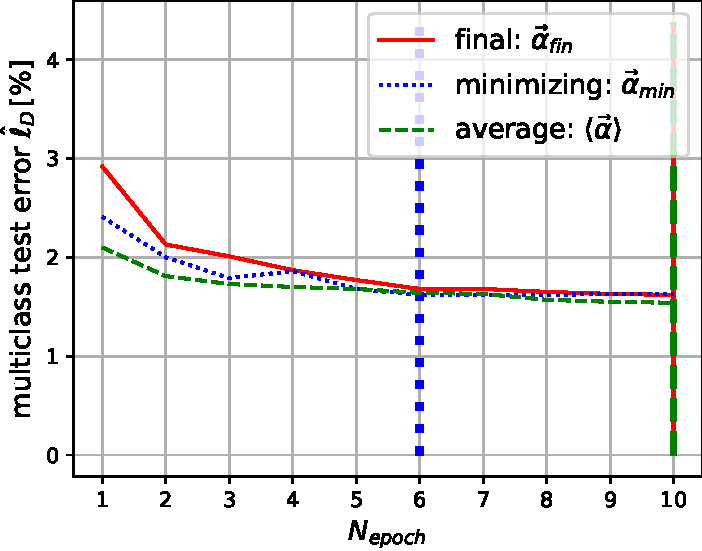
\includegraphics[width=\linewidth]{performance/test_deg=4.pdf} 
        \caption{$p = 4$}
    \end{subfigure}
    \par\bigskip
        \begin{subfigure}[t]{0.49\textwidth}
        \centering
        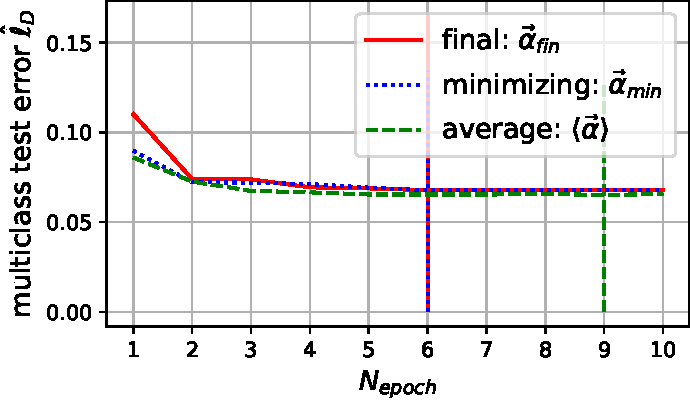
\includegraphics[width=\linewidth]{performance/test_deg=5.pdf} 
        \caption{$p = 5$}
    \end{subfigure}
    \hfill
    \begin{subfigure}[t]{0.49\textwidth}
        \centering
        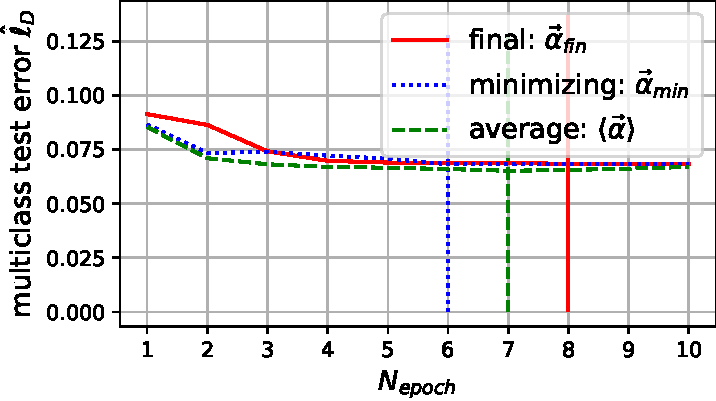
\includegraphics[width=\linewidth]{performance/test_deg=6.pdf} 
        \caption{$p = 6$}
    \end{subfigure}
    \caption{test error rates}
\end{figure}

\begin{figure}
\centering
	\begin{subfigure}[t]{0.49\textwidth}
	\centering
		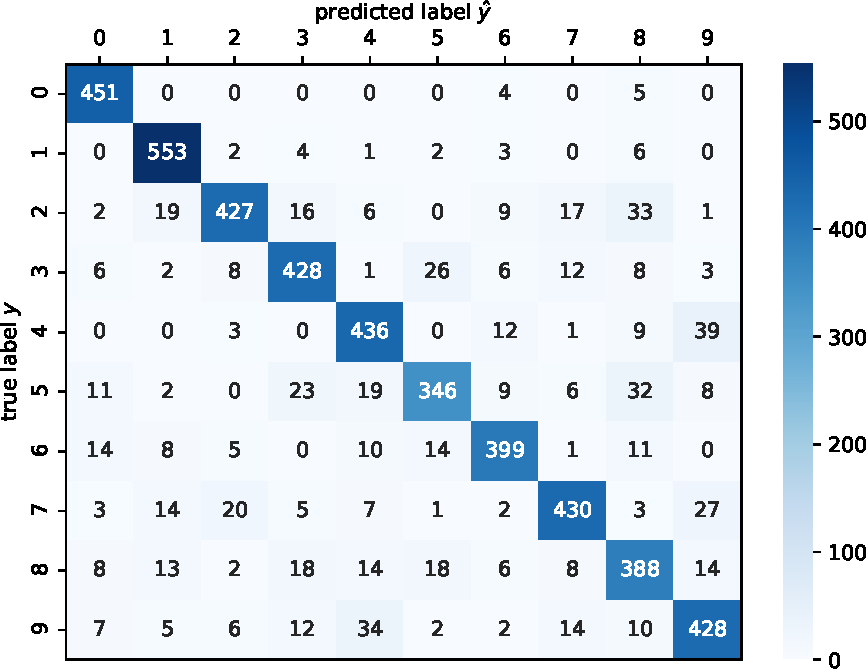
\includegraphics[width=\linewidth]{conf_mat/predictor.pdf} 
		\caption{final predictor $\vec{\alpha}_{fin}$}
	\end{subfigure}
	\hfill
	\begin{subfigure}[t]{0.49\textwidth}
	\centering
		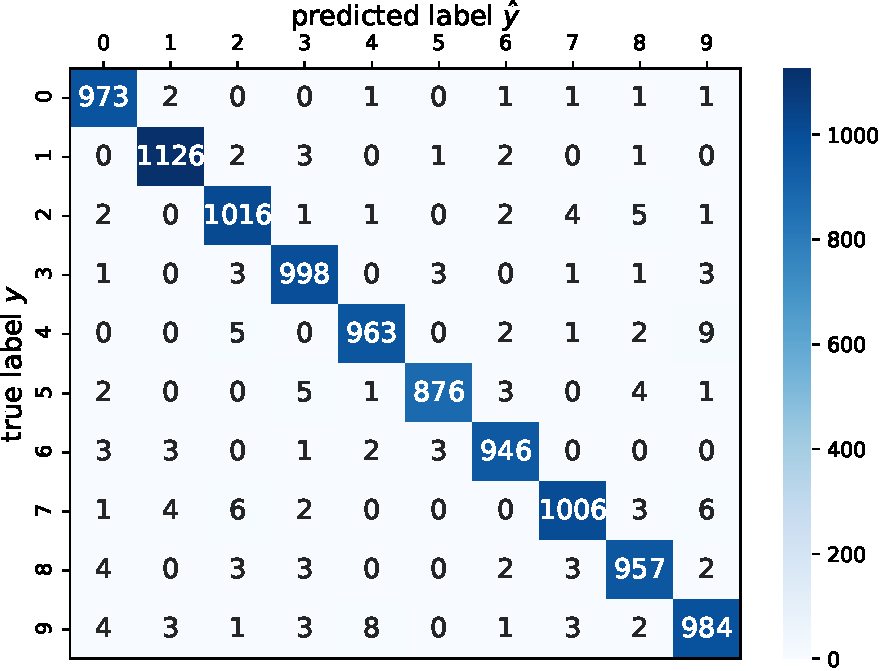
\includegraphics[width=\linewidth]{conf_mat/min_predictor.pdf} 
		\caption{minimizing predictor $\vec{\alpha}_{min}$}
	\end{subfigure}
		\begin{subfigure}[t]{0.49\textwidth}
	\centering
		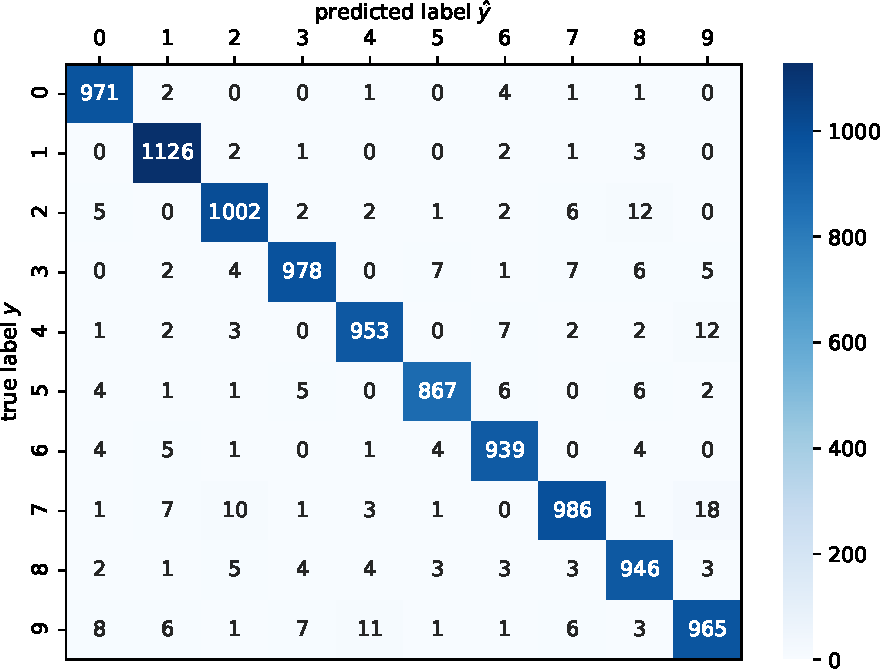
\includegraphics[width=\linewidth]{conf_mat/avg_predictor.pdf} 
		\caption{minimizing predictor $\langle\vec{\alpha}\rangle$}
	\end{subfigure}
\end{figure}

\subsection{Minimizing the Test Error Rate}\label{subsec:best_pred}
